\chapter{PLANTEAMIENTO DEL PROBLEMA}
\section{Descripción de la Realidad Problemática}

Desde inicios de la historia, las enfermedades infecciosas hasta crónicas han sido parte de la humanidad y han afectado desde pueblos hasta naciones. No obstante, gracias al avance de la medicina se a podido comprender muchas de estas enfermedades, logrando mejorar la salud de muchas personas o su completa recuperación. Pero en el mejor de los casos eliminada o controlada por completo, el caso más conocido es la viruela que fue erradicada en 1980 debido a un programa mundial de vacunación. 


\begin{figure}[h]
	\begin{center}
		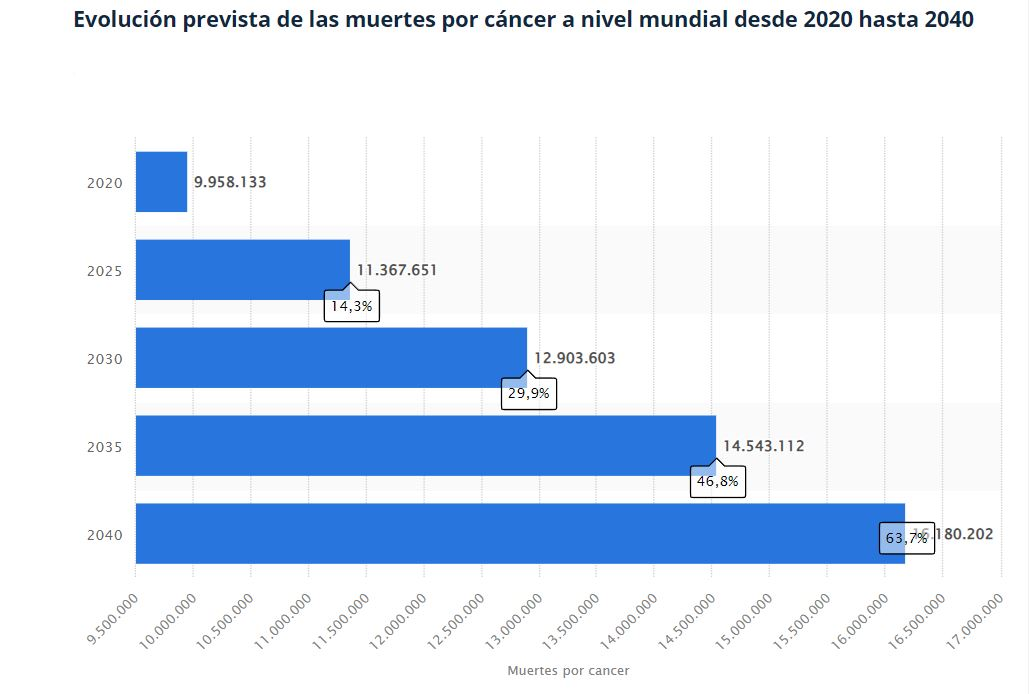
\includegraphics[width=0.75\textwidth]{1/figures/Grafico1DiagnosnitoCancer.JPG}
		\caption{Predicción de número de casos acumulado de cancer a nivel mundial. Fuente: \cite{stadisitc_cancer}}
		\label{1:fig}
	\end{center}
\end{figure}


Sin embargo, una enfermedad que ha afectado durante siglos a la humanidad es el cáncer. Este se caracteriza por su capacidad de alterar el equilibrio de las células del cuerpo humano, provocando un crecimiento anormal y descontrolado de las zonas afectadas a tal grado que puede llegar a invadir otras partes del cuerpo. La Organización mundial de la salud (OMS) afirma que el cáncer es la segunda causa muerte más frecuente en América y una las principales a nivel mundial. En estima que en el año 2022 hubo 20 millones de nuevos casos y 9,7 millones de muertes. Como se pude observar en la figura\ref{1:fig}, según el estudio de Statista publicado en el año 2023 se proyecta que el número de nuevos casos de cáncer crecerá notoriamente en los próximos 20 años.\parencite{OMS_cancer}






Entre los tipos más comunes de cáncer se encuentra el que afecta a la piel el cual se puede contraer a cualquier edad; sin embargo, las personas de mayor riesgo son las que estan expuestos por tiempos prolongados al sol y poseen piel clara. La principal causa es la exposición a la radiación ultravioleta o fuentes artificiales. Según American Cancer Society para el año 2023 morirán aproximadamente que morirán aproximadamente 7,990 personas y aproximadamente aparecerán 97,610 nuevos casos.

Si bien la mayoría de los casos se puede tratar sin complicaciones, existe un porcentaje en el cual puede llegar a ser peligro y potencialmente mortal. Esto principalmente debido a que no es detectado a tiempo o no se cuenta con dermatólogos especializados en esta área.

\begin{figure}[h]
	\begin{center}
		\includegraphics[width=0.5\textwidth]{1/figures/radiación_ultravioleta_peru.png}
		\caption{Pronóstico de radiación UV. Fuente: \cite{SENAMHI_uv}}
		\label{1:fig1}
	\end{center}
\end{figure}



En el caso del Perú, el cáncer de piel está en aumento, especialmente debido a la alta incidencia de radiación ultravioleta (UV) en muchas regiones del país como podemos ver en la figura\ref{1:fig1} el nivel de radiacion ultravioleta el dia 21 de abril del 2024 \parencite{SENAMHI_uv}  y la falta de conciencia sobre la protección solar adecuada. Agregando, la detección temprana y el tratamiento oportuno de esta enfermedad son difíciles por la falta de acceso a servicios de salud especializados en algunas áreas rurales y remotas. Como podemos observar en la siguente figura\ref{1:fig2} La cual nos indica que el 73\%\ de los casos fueron cuando acudieron a un establecimiento de salud en el momento que ya presentaron síntomas muy notorios de cáncer, haciendo evidencia de que el fue diagnosticado de forma tardía. \parencite{cancer_diagnostico}



\begin{figure}[h]
	\begin{center}
		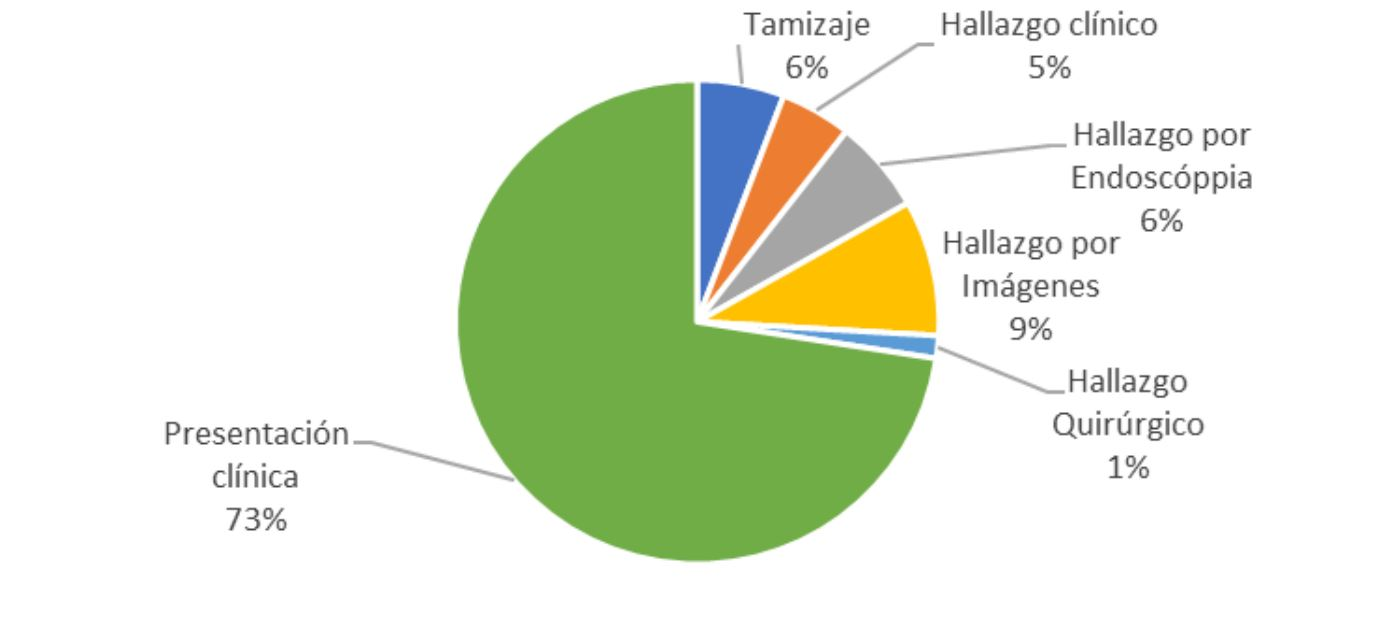
\includegraphics[width=0.8\textwidth]{1/figures/cancer_diagnostico.JPG}
		\caption{Metodo del primer diagnostico DEL CANCER.PERU 2019-2022: \cite{cancer_diagnostico}}
		\label{1:fig2}
	\end{center}
\end{figure}







\section{Formulación del Problema}

Para realizar la formulación de los problemas del presente trabajo, se elaboró una  Matriz de Consistencia (Anexo \ref{anebxo1}).

\subsection{Problema General}
\newcommand{\ProblemaGeneral}{ Dificultad de detección temprana de cáncer de piel en el Perú debido a la falta de especialistas en esa área}
\ProblemaGeneral
\subsection{Problemas Espec\'{i}ficos}
\newcommand{\Pbone}{
¿Cuáles son los algoritmos de Deep Learning que pueden clasificar con precisión los melanomas y no melanomas entre pacientes peruanos?
}
\newcommand{\Pbtwo}{
¿Cuál es el desafío principal entre reconocer los tipos de cáncer en los pacientes peruanos?
}
\newcommand{\Pbthree}{
¿Qué tipo de ruido pude haber en la imagenes que dificulté la clasificación de los melanomas y no melanomas entre pacientes peruanos?
}
\newcommand{\Pbfour}{
¿ Qué alternativas se proponen en los trabajos previos para seleccionar características y desarrollar el marco de trabajo de la investigación?
}
\newcommand{\Pbfive}{
¿Cuál es la influencia de las condiciones ambientales y geográficas específicas de Perú en el tratamiento del cáncer de piel?
}

\begin{itemize}
	\item \Pbone
	\item \Pbtwo
	\item \Pbthree
	\item \Pbfour
	\item \Pbfive
\end{itemize}

\section{Objetivos de la Investigación}

Para realizar la formulación de los problemas del presente trabajo, se elaboró una  Matriz de Consistencia (Anexo \ref{anexo1}).


\subsection{Objetivo General}
\newcommand{\ObjetivoGeneral}{
Determinar cuál de las herramientas propuestas en los trabajos previos es la más precisa y confiable en la detección utilizando imágenes dermatoscopias de pacientes peruanos

}
\ObjetivoGeneral
\subsection{Objetivos Espec\'{i}ficos}
\newcommand{\Objone}{
Identificar y comparar los algoritmos de Deep Learning más adecuados para la clasificación de melanomas y no melanomas en imágenes dermatoscópicas de pacientes del Perú.
}
\newcommand{\Objtwo}{
Analizar cómo las características dermatoscópicas únicas en Perú afectan el reconocimiento de melanomas y no melanomas de pacientes del Perú.
}
\newcommand{\Objthree}{
Identificar y evaluar el impacto de estos ruidos en la precisión de la clasificación de melanomas y no melanomas de pacientes del Perú.
}
\newcommand{\Objfour}{
Analizar los diferentes enfoques utilizados en investigaciones anteriores con la finalidad de desarrollar marcos de trabajo efectivos para la clasificación de melanomas y no melanomas de pacientes del Perú.
}
\newcommand{\Objfive}{
Analizar cómo as condiciones ambientales y geográficas pueden afectar los melanomas y no melanomas de pacientes del Perú.
}

\begin{itemize}
	\item {\Objone}
	\item {\Objtwo}
	\item {\Objthree}
	\item {\Objfour}
	\item {\Objfive}
\end{itemize}

\section{Justificación de la Investigación}

\subsection{Teórica}
Esta investigación se realiza 

\subsection{Práctica}
Al culminar la investigación 

\subsection{Metodológica}. 

\section{Delimitación del Estudio}

\subsection{Espacial}
Para la presente investigación 

\subsection{Temporal}
Los datos que serán necesari. 

\subsection{Conceptual}
Esta investigación se 

\section{Hipótesis}

\subsection{Hipótesis General}
\newcommand{\HipotesisGeneral}{
El uso de técnicas de.
}
\HipotesisGeneral
\subsection{Hipótesis Específicas}
\newcommand{\Hone}{
	x
}
\newcommand{\Htwo}{
	y
}
\newcommand{\Hthree}{
	z	
}
\newcommand{\Hfour}{
	cv
}
\newcommand{\Hfive}{
	xws
}
\begin{itemize}
	\item \Hone
	\item \Htwo
	\item \Hthree
	\item \Hfour
	\item \Hfive
\end{itemize}

\subsection{Matriz de Consistencia}
A continuación se presenta la matriz de consistencia elaborada para la presente investigación (véase Anexo \ref{1:table}).

